\documentclass[a4paper,11pt]{article}
\usepackage{mathtools}
\usepackage[T1]{fontenc}
\usepackage[utf8]{inputenc}
\usepackage{graphicx}
\usepackage{xcolor}
\usepackage{verbatim}
\usepackage{amsmath}
\usepackage{array}
\usepackage{amssymb}
\usepackage{mathtools}
\usepackage{graphicx}
\usepackage{epstopdf}
\usepackage{inputenc}
\usepackage{breqn}
\usepackage{geometry}
\usepackage[linesnumbered,ruled]{algorithm2e}
\usepackage{amsmath}
\usepackage{amsmath,amssymb}
\usepackage{bm}
\usepackage{eqparbox}
\DeclareMathOperator{\E}{\mathbb{E}}
\usepackage{etoolbox}  % patch def of algorithmic environment
\makeatletter
\patchcmd{\algorithmic}{\addtolength{\ALC@tlm}{\leftmargin} }{\addtolength{\ALC@tlm}{\leftmargin}}{}{}
\makeatother
\usepackage[
pdftitle={Assignment 4}, 
pdfauthor={Yash Gangrade, University of Utah},
colorlinks=true,linkcolor=black,urlcolor=blue,citecolor=blue,bookmarks=true, bookmarksopenlevel=2]{hyperref}
\usepackage{amsmath,amssymb,amsthm,textcomp}
\usepackage{enumerate}
\usepackage{multicol}
\usepackage{tikz}
\usepackage{imakeidx}
\makeindex[columns=3, title=Alphabetical Index, intoc]
\usepackage{geometry}
\usepackage{algorithm, algorithmicx, algpseudocode}
\usepackage{mdframed}
\geometry{total={210mm,297mm},
left=20mm,right=20mm,%
bindingoffset=0mm, top=20mm,bottom=20mm}

\linespread{1.1}
\DeclareUnicodeCharacter{2212}{\in} 
\newcommand{\linia}{\rule{\linewidth}{0.5pt}}
\newcommand\Myperm[2][^n]{\prescript{#1\mkern-2.5mu}{}P_{#2}}
\newcommand\Mycomb[2][^n]{\prescript{#1\mkern-0.5mu}{}C_{#2}}
% custom theorems if needed
\newtheoremstyle{mytheor}
    {1ex}{1ex}{\normalfont}{0pt}{\scshape}{.}{1ex}
    {{\thmname{#1 }}{\thmnumber{#2}}{\thmnote{ (#3)}}}

\theoremstyle{mytheor}
\newtheorem{defi}{Definition}

\graphicspath{{Figures/}}

% my own titles
\makeatletter
\renewcommand{\maketitle}{
\begin{center}
\vspace{2ex}
{\huge \textsc{\@title}}
\vspace{1ex}
\\
\linia\\
\@author \hfill \@date
\vspace{4ex}
\end{center}
}
\makeatother
%%%

% custom footers and headers
\usepackage{fancyhdr,lastpage}
\pagestyle{fancy}
\lhead{}
\chead{}
\rhead{}
\lfoot{Assignment \textnumero{} 4}
\cfoot{}
\rfoot{Page \thepage\ of \ \pageref*{LastPage}}
\renewcommand{\headrulewidth}{0pt}
\renewcommand{\footrulewidth}{0pt}
%

%%%----------%%%----------%%%----------%%%----------%%%

\begin{document}

\title{CS 6635: Visualization of Scientific Data Homework 4 \\ \large Multi Field Visualization}

\author{Yash Gangrade (u1143811), MS First Year, School of Computing}

\date{25\textsuperscript{th} March 2018}
\maketitle
\tableofcontents
\listoffigures
\null \clearpage

%%%%%%%%%%%%%%%%%%% Main Content %%%%%%%%%%%%%%%%%%%
%%%%%%%%%%%%%%%%%%% Part I %%%%%%%%%%%%%%%%%%%
%%%%%%% Question 1 %%%%%%%
\section{Part 1 - Scalar Field Visualization}
\subsection{Create isosurfaces of both QCLOUD and the magnitude of the Wind.}
\paragraph{Ans.}
As this is the scalar field simulation, we are using contour filter (essentially isosurface) to visualize the QCLOUD and Wind Magnitude Isosurface. One of the main things before starting to solve the problem was to enable the "Auto Convert Properties" in the settings of Paraview. After doing this, we were able to get specific properties like Wind\_Magnitude, Wind\_X, etc. Now to get the QCLOUD Isosurface, we first started with the lowest iso-surface value and then kept modifying it by changing it by factor size of 2 until we get reasonable visualizations. Also, in the next question, it asks to change the colors and opacity for one of the iso-surfaces. You can find the results below. For QCLOUD, I am using the iso-value of 2.02947e-6 to get the required visualization. Similarly, to get the iso-surface of Wind Magnitude, we changes the contour by property to wind\_magnitude and the iso-value for that to 12.452. The results for both the cases are attached below. Please feel free to have a look at Part1.pvsm or the screenshots of settings in Images folder of zip file attached. 

\begin{figure}[!h]
    \centering
    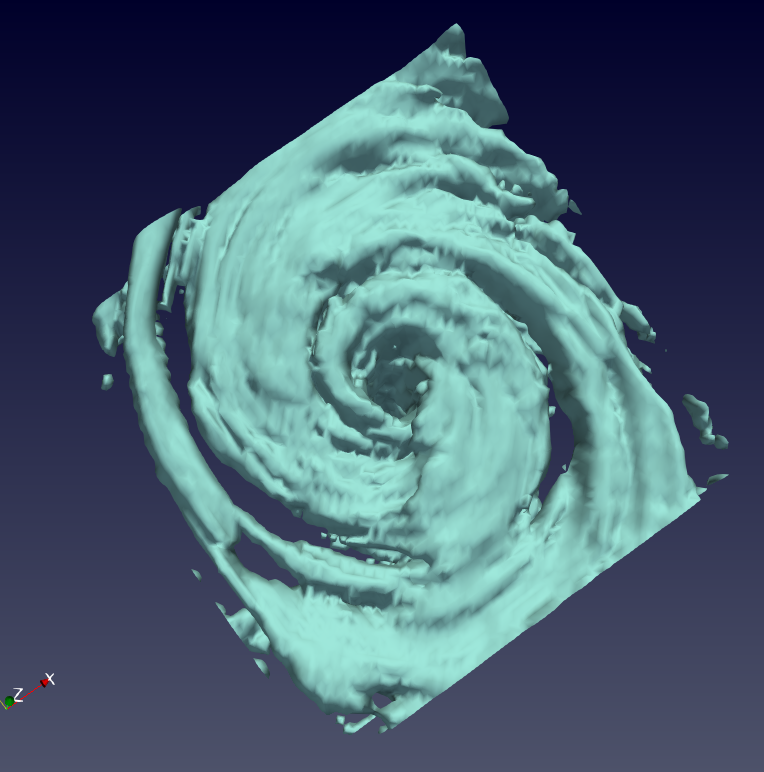
\includegraphics[scale=0.4]{Figures/P1_3_1.PNG}
    
    \vspace{1 cm}
    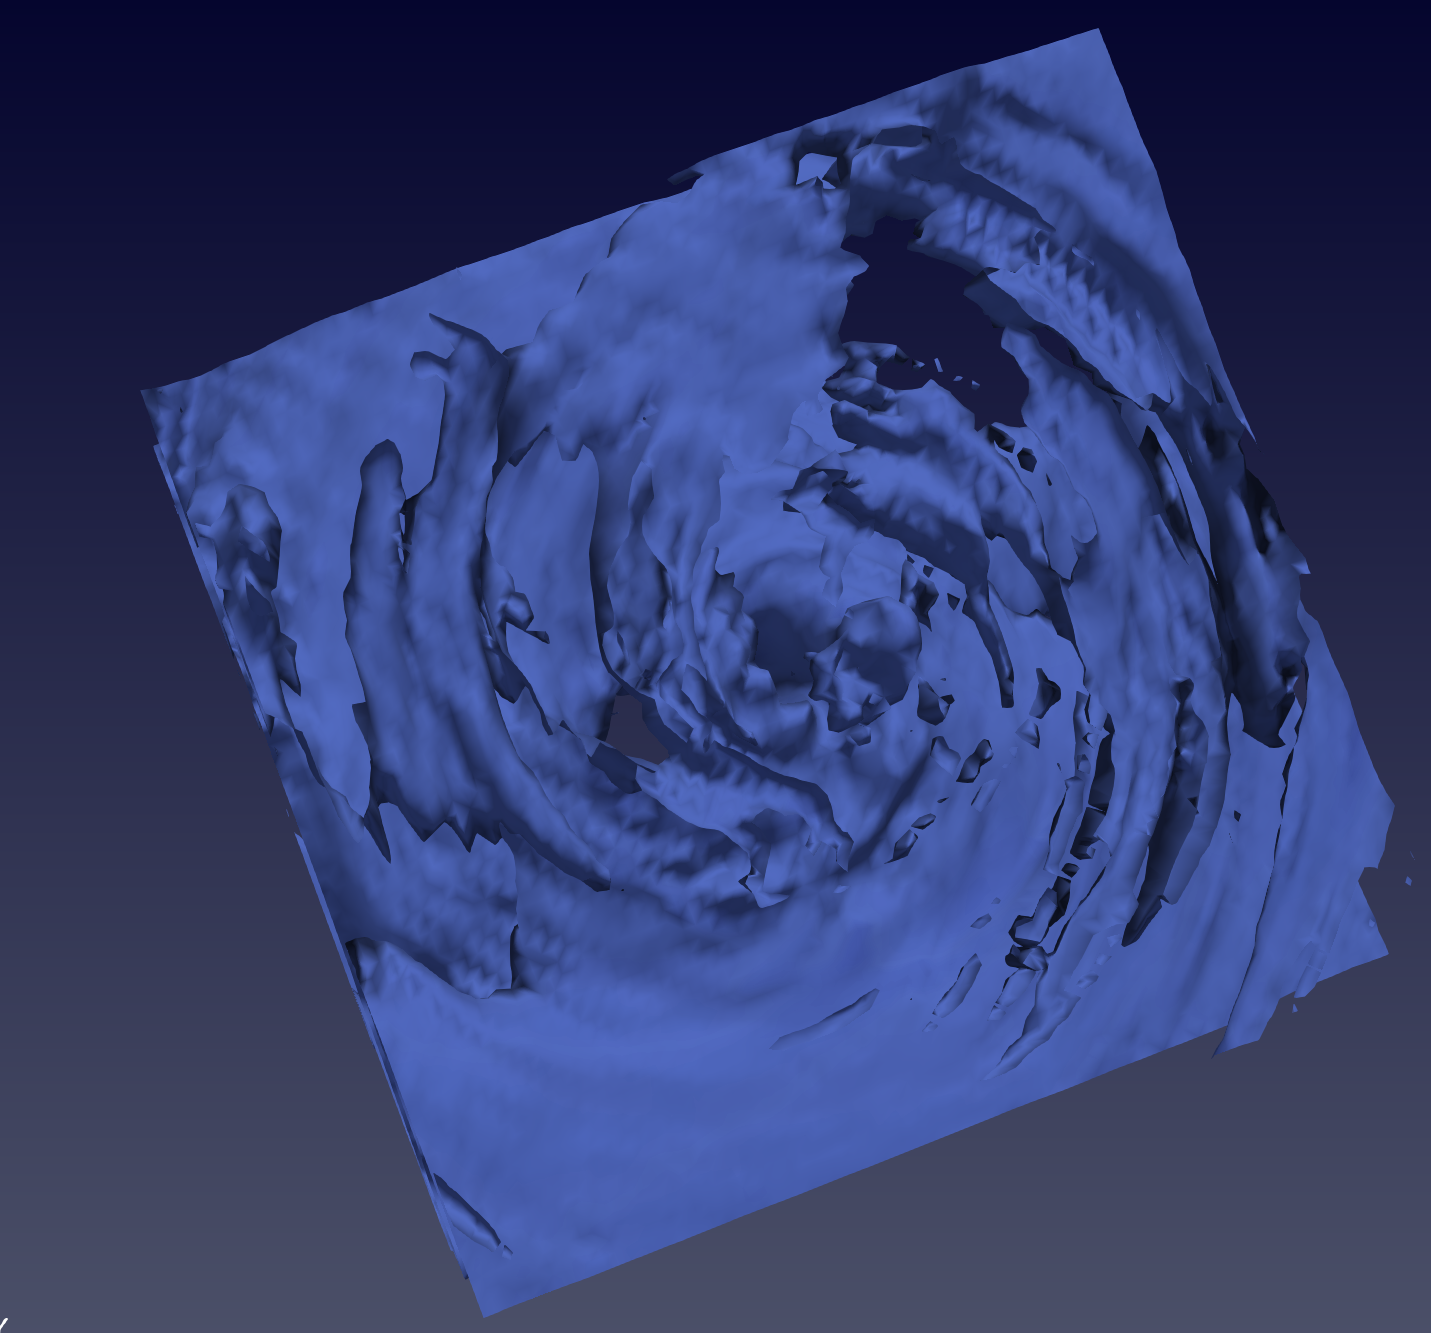
\includegraphics[scale=0.4]{Figures/P1_1_2.PNG}
    \caption{Top: QCLOUD Isosurface, Bottom: Wind Isosurface}
    \label{p1_1}
\end{figure}
\clearpage
The settings to get the required iso-surfaces are attached in form of screenshots below.

\begin{figure}[!h]
    \centering
    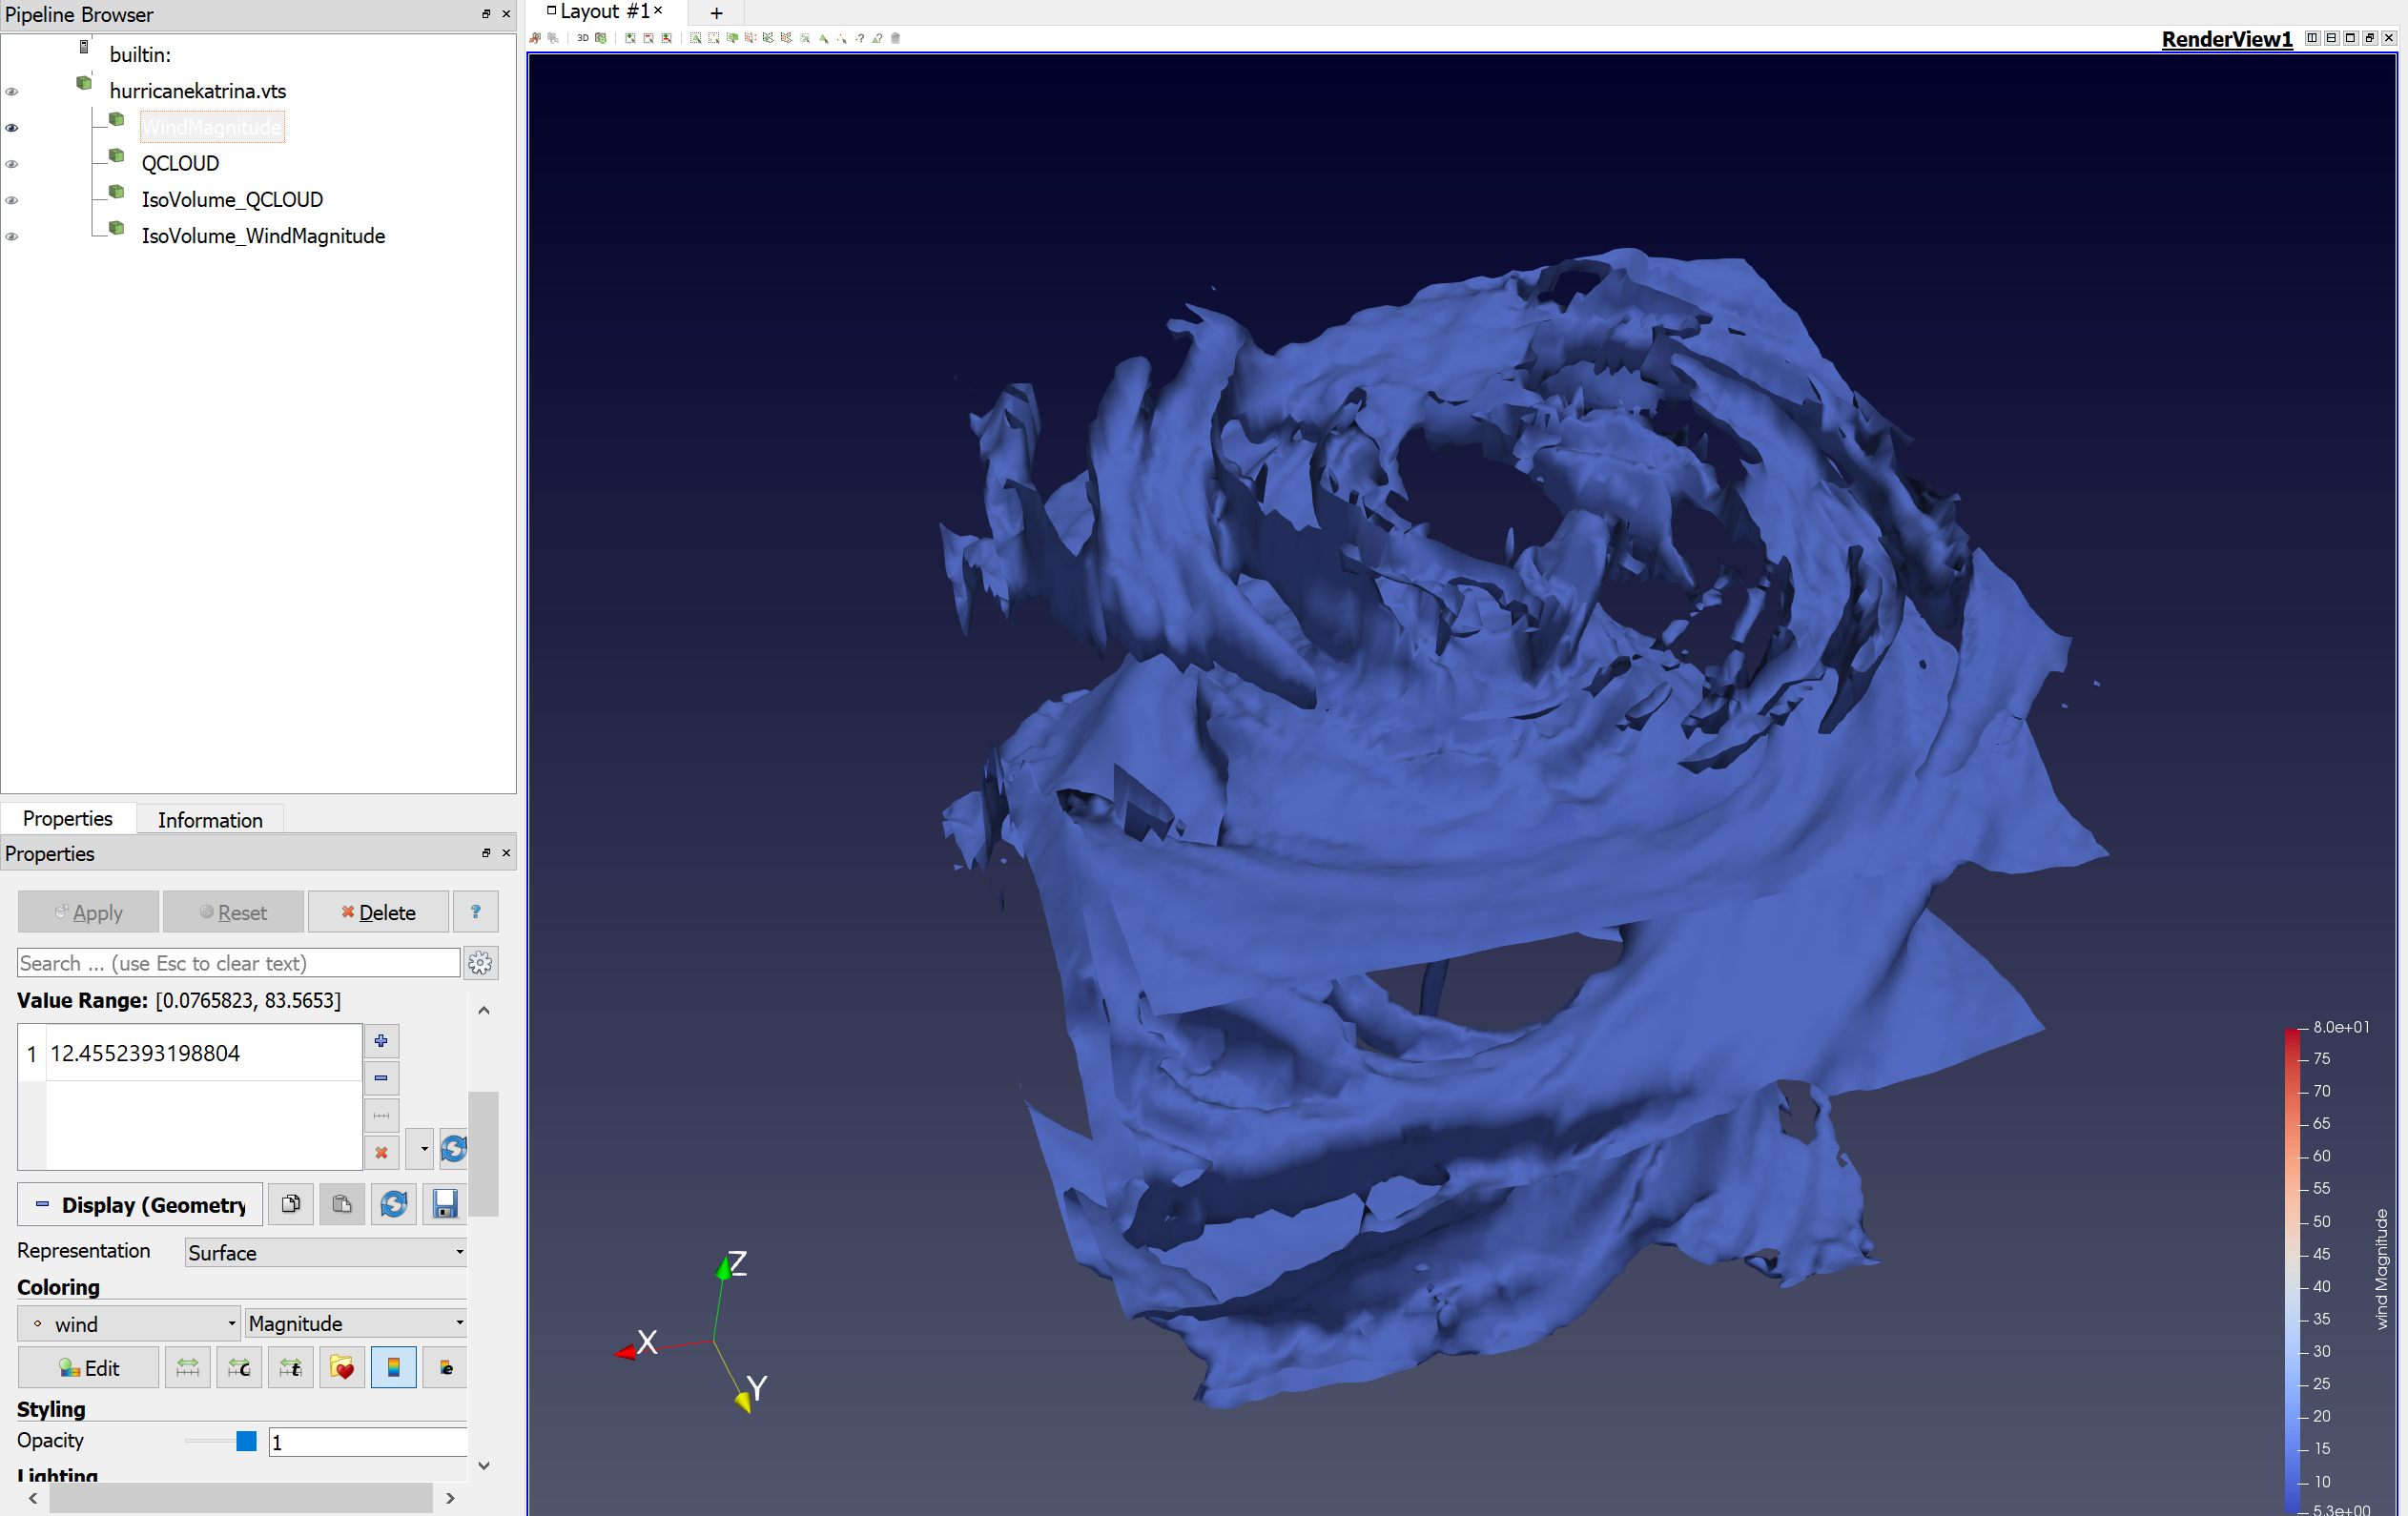
\includegraphics[scale=0.45]{Figures/P1_1_1.PNG}
    
    \vspace{1 cm}
    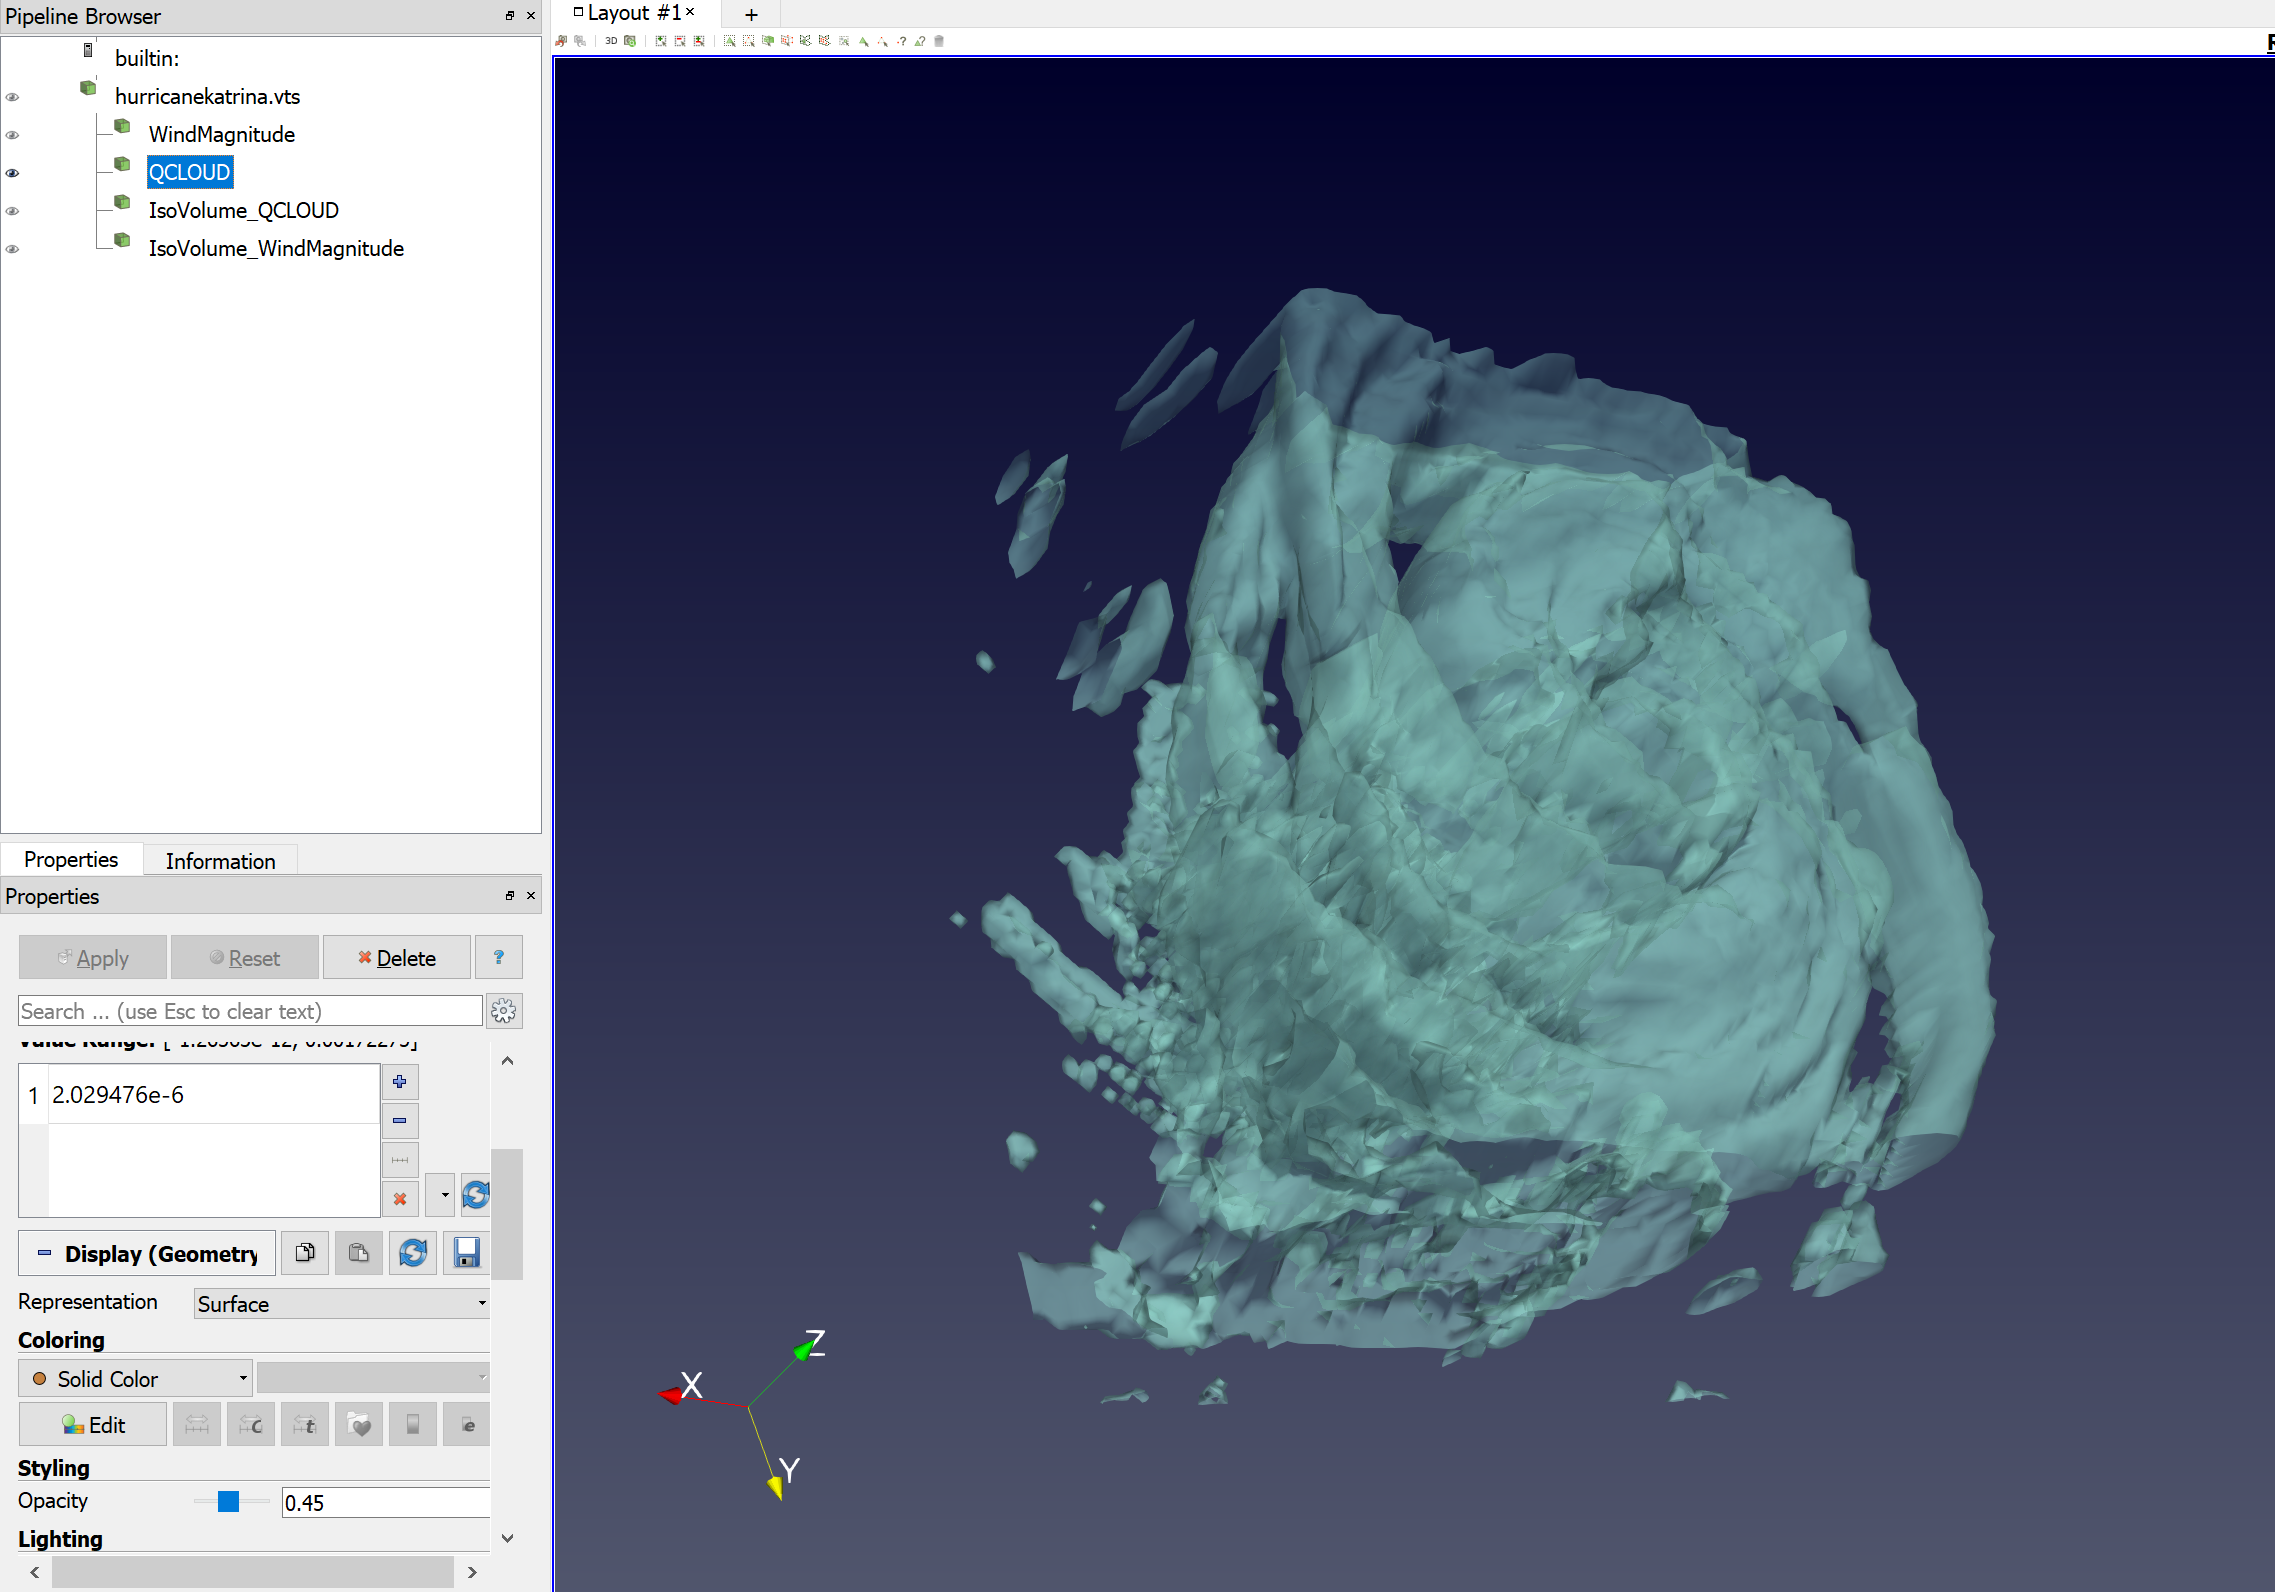
\includegraphics[scale=0.5]{Figures/P1_2_1.PNG}
    \caption{Top: Wind Isosurface Settings, Bottom: QCLOUD Isosurface Settings}
    \label{p1_6}
\end{figure}

\clearpage

\subsection{Color the two isosurfaces and make one of them partially transparent.}
\paragraph{Ans.} I decided to make the QCLOUD Iso-surface transperent by changing it's opacity to 0.45. Also, the visualization with both the iso-surfaces together is shown below. Here, it can be clearly seen that the wind flow is following the cloud iso-surface as expected. 
\begin{figure}[!h]
    \centering
    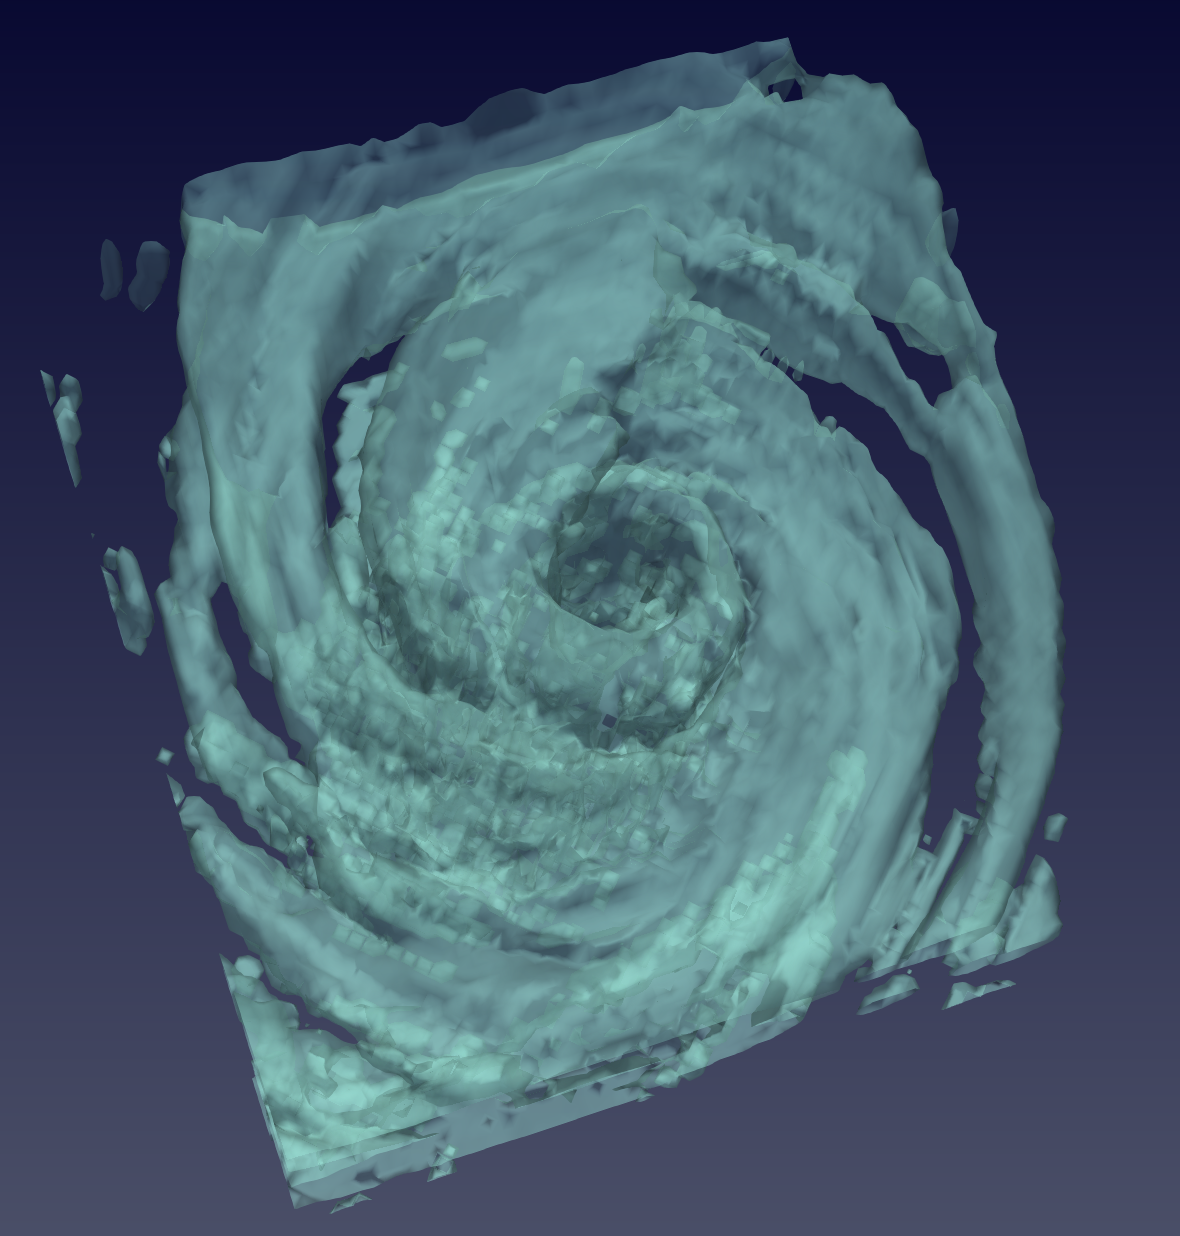
\includegraphics[scale=0.6]{Figures/P1_2_2.PNG}
    
    \vspace{1 cm}
    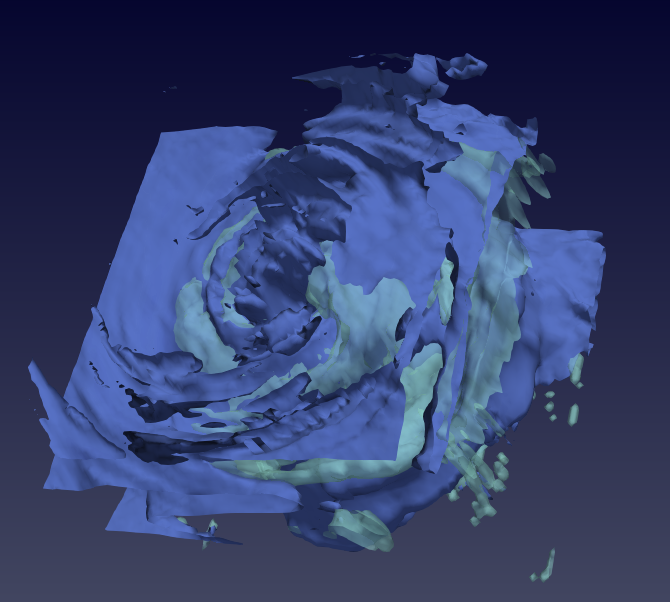
\includegraphics[scale=0.56]{Figures/P1_3_2.PNG}
    \caption{Top: QCLOUD Isosurface (Opacity = 0.45), Bottom: QCLOUD and Wind Maginitude Isosurfaces together}
    \label{p1_2}
\end{figure}

\subsection{Create separate volume renderings of both QCLOUD and the magnitude of the
Wind Speed. Create transfer functions that show the higher wind speeds near the
center of the hurricane.}
\paragraph{Ans.} We used the iso-volume filters in paraview to create the iso-volume rendering of QCLOUD and Wind Speed. Firstly, for the QCLOUD Isovolume, we used the range [1.723e-5, 1.723e-3] of iso-values to get the required volume rendering. The transfer function of QCLOUD is also modified so as to get a reasonable visualization of the volume rendering. Please find the attached screenshot of settings to know the transfer function used. Similarly, for the iso-volume of the magnitude of the wind, we used the iso-value range as [14.27, 33.47]. The transfer function is also modified such that the higher wind speeds are shown at the center of the hurricane. We know that this is a scalar field visualization. In wind magnitude volume rendering, we can see the varying magnitude of wind speeds at different locations of hurricane, especially the higher wind speeds at the epicenter of the hurricane. The resultant diagrams are attached below. 

\begin{figure}[!h]
    \centering
    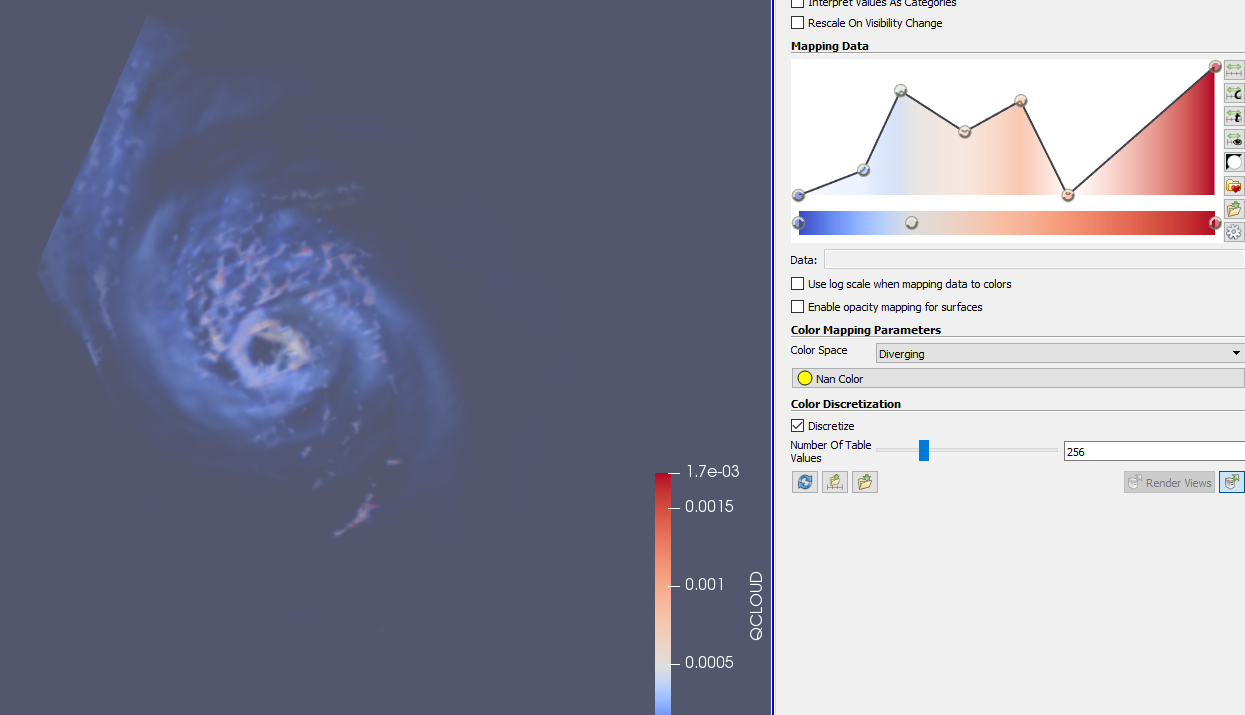
\includegraphics[scale=0.5]{Figures/P1_4_5.PNG}
    \caption{QCLOUD Iso-volume rendering with modified transfer function, higher wind speeds can be visualized at the center}
    \label{p1_3}
\end{figure}
\clearpage

\begin{figure}[!h]
    \centering
    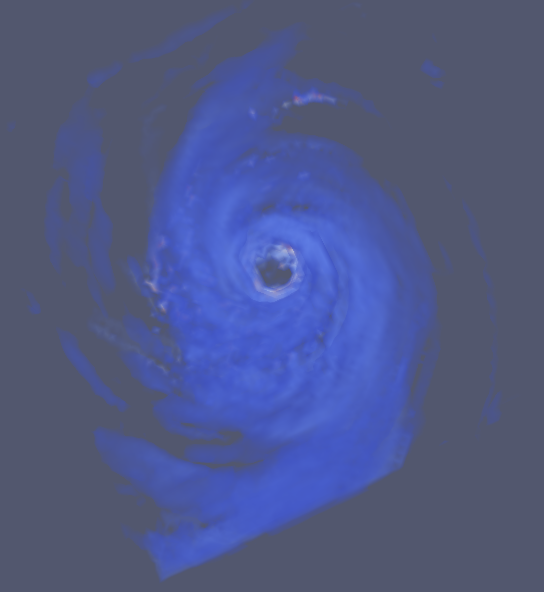
\includegraphics[scale=0.8]{Figures/P1_4_1.PNG}
    
    \vspace{0.5 cm}
    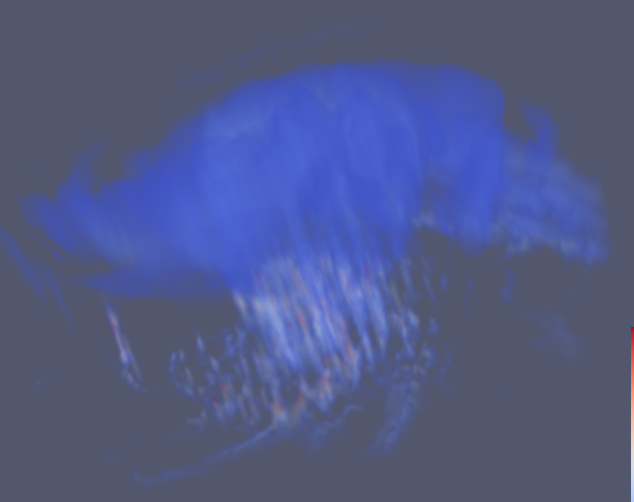
\includegraphics[scale=0.8]{Figures/P1_4_2.PNG}
    \caption{Different views of iso-volume rendering of QCLOUD}
    \label{p1_4}
\end{figure}
\clearpage

\begin{figure}[!h]
    \centering
    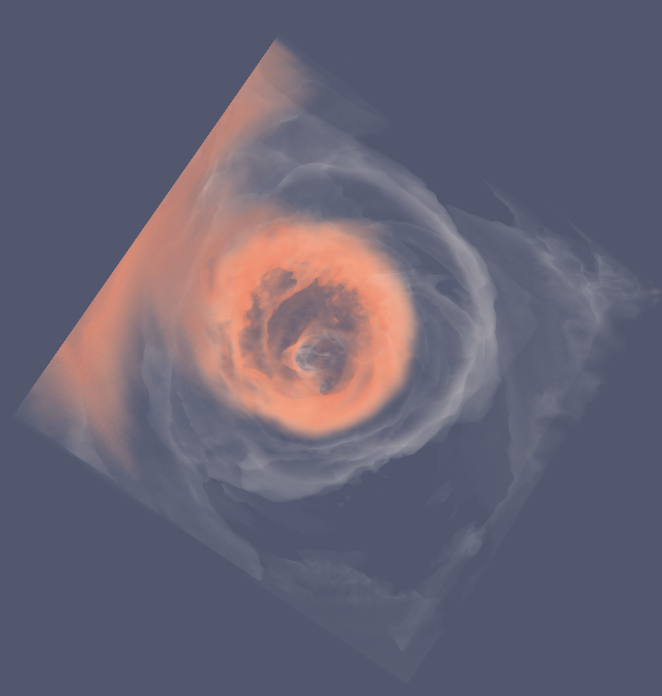
\includegraphics[scale=0.8]{Figures/P1_4_3.PNG}
    
    \vspace{0.5 cm}
    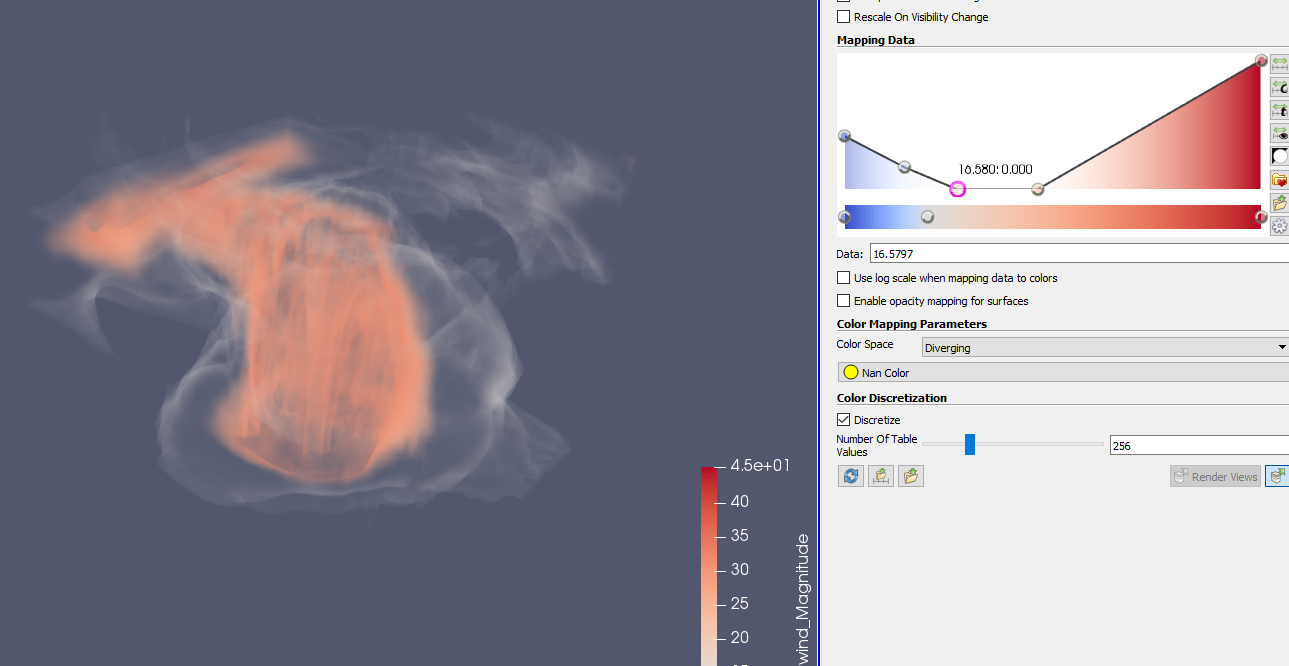
\includegraphics[scale=0.5]{Figures/P1_4_4.PNG}
    \caption{Top: Iso-volume rendering of wind speed, Bottom: Modified Transfer Function to show higher wind speeds near the center of the hurricane}
    \label{p1_5}
\end{figure}


\clearpage

\section{Part 2 - Vector Field Visualization}
\subsection{Create streamlines of the wind flow within the hurricane. Seed the streamlines so as to
get a good overview of the flow.}
\paragraph{Ans.} Here, we used the stream tracer filter upon the wind flow in the hurricane dataset. To get a reasonable visualization of the streamlines, I changed the seed line a lot so as to make the hurricane epicenter area narrow. Also, as it is clearly evident from the results, this visualization indeed looks like a hurricane visualization. To make a clear view, I changed the resolution of stream tracer filter to 180 (default is 1000). In fig. \ref{p2_1}b we can see that the streamlines follow the iso-volume rendering properly and this view gives us a better understanding of the dataset. It gives us a rough idea of how the wind is flowing inside the hurricane. The results from the stream tracer filter are attached below. 

\begin{figure}[!h]
    \centering
    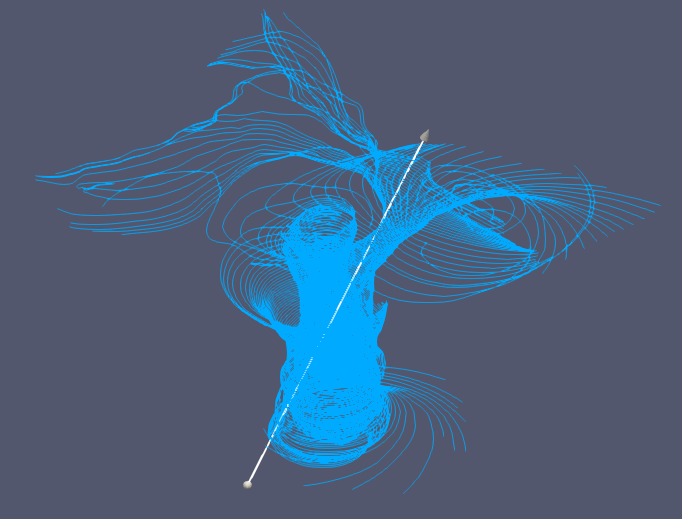
\includegraphics[scale=0.6]{Figures/P2_1_1.PNG}
    
    \vspace{1 cm}
    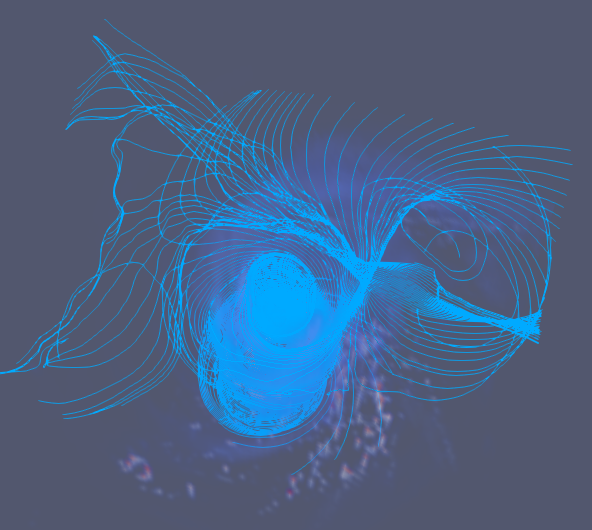
\includegraphics[scale=0.56]{Figures/P2_1_2.PNG}
    \caption{Top: Streamlines of the wind flow, Bottom: Streamlines of the wind flow and IsoVolume Rendering of the wind magnitude together}
    \label{p2_1}
\end{figure}

\clearpage
\subsection{Create stream tubes of the wind flow within the hurricane.}
\paragraph{Ans} One of the important thing here to note is that the tube filter should be added to the streamlines and not to the hurricane dataset. I made this mistake and wasted about an hour, later realizing why visualization is wrong here. Essentially, stream tubes are same as stream lines but the tubes gives us a better visualization as compared to the stream tracer. One thing I found was that it is opaque and thus provides a much clearer view. Here, to make the visualization better, I changed the radius of the tubes to $\sim$4000 and the radius factor to 5. I really found this visualization very interesting. It seems much better than streamlines in providing the information about the dataset. This helped me understand the shapee of hurricane near the epicenter. The resultant figure is as shown below. 

\begin{figure}[!h]
    \centering
    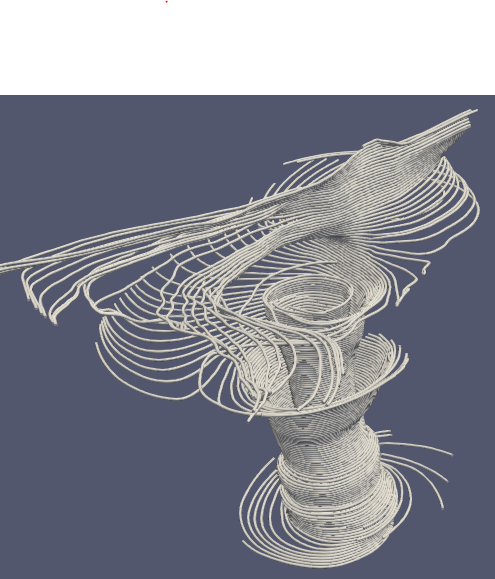
\includegraphics[scale=0.6]{Figures/P2_2_1.PNG}
    \caption{Stream Tubes applied to Streamlines}
    \label{p2_2}
\end{figure}

\clearpage

\subsection{Add cone glyphs to the stream tubes so you can see direction of the flow.}
Here, we added a glyph filter to the stream tubes we had. One of the important thing to note is that, paraview crashes if you use the default settings of glyphs. I changed the glyph mode to "Every Nth point" instead of "Uniform Spatial Distributions". Also, we are using every point out of 1000 sampled points i.e. the sampling rate is 1000. I also changed the Scale Mode to vector and the scale factor to $\sim$21000. For coloring, I changed the color type to GlyphVector to represent both magnitude and direction. Finally, change the type of glyph to cone and hit apply. Through this view, we can see the wind flow and directions along the streamlines. For better visualization, I enabled the stream tubes and the glyphs together to get an understanding of the data. From the results attached below we can clearly see the direction of the wind flow and magnitude along the stream tubes. 

\begin{figure}[!h]
    \centering
    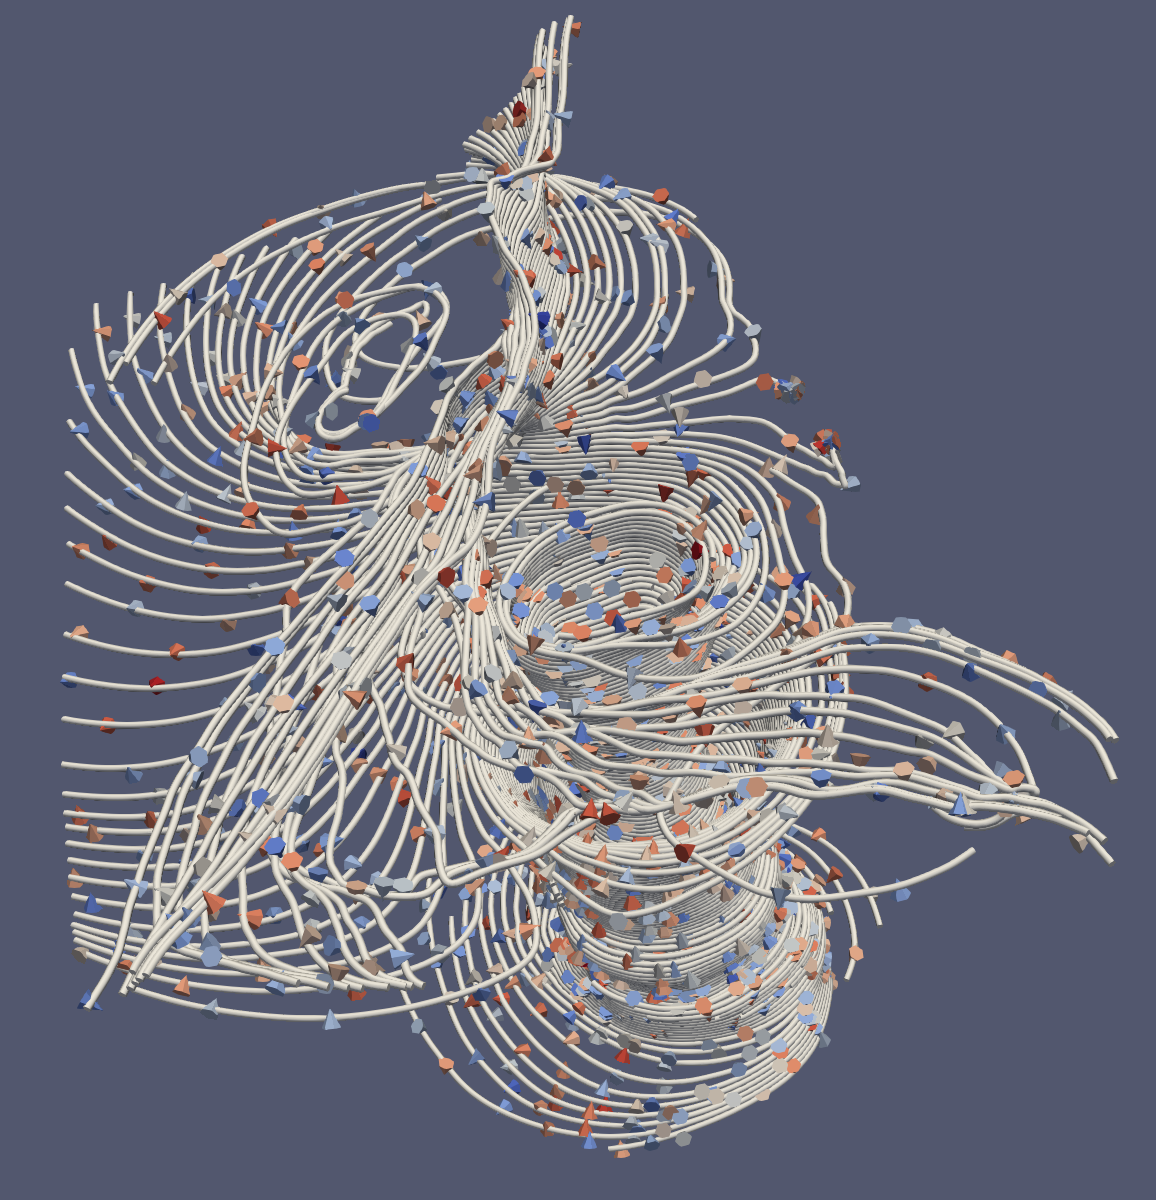
\includegraphics[scale=0.5]{Figures/P2_3_1.PNG}
    
    \vspace{0.5 cm}
    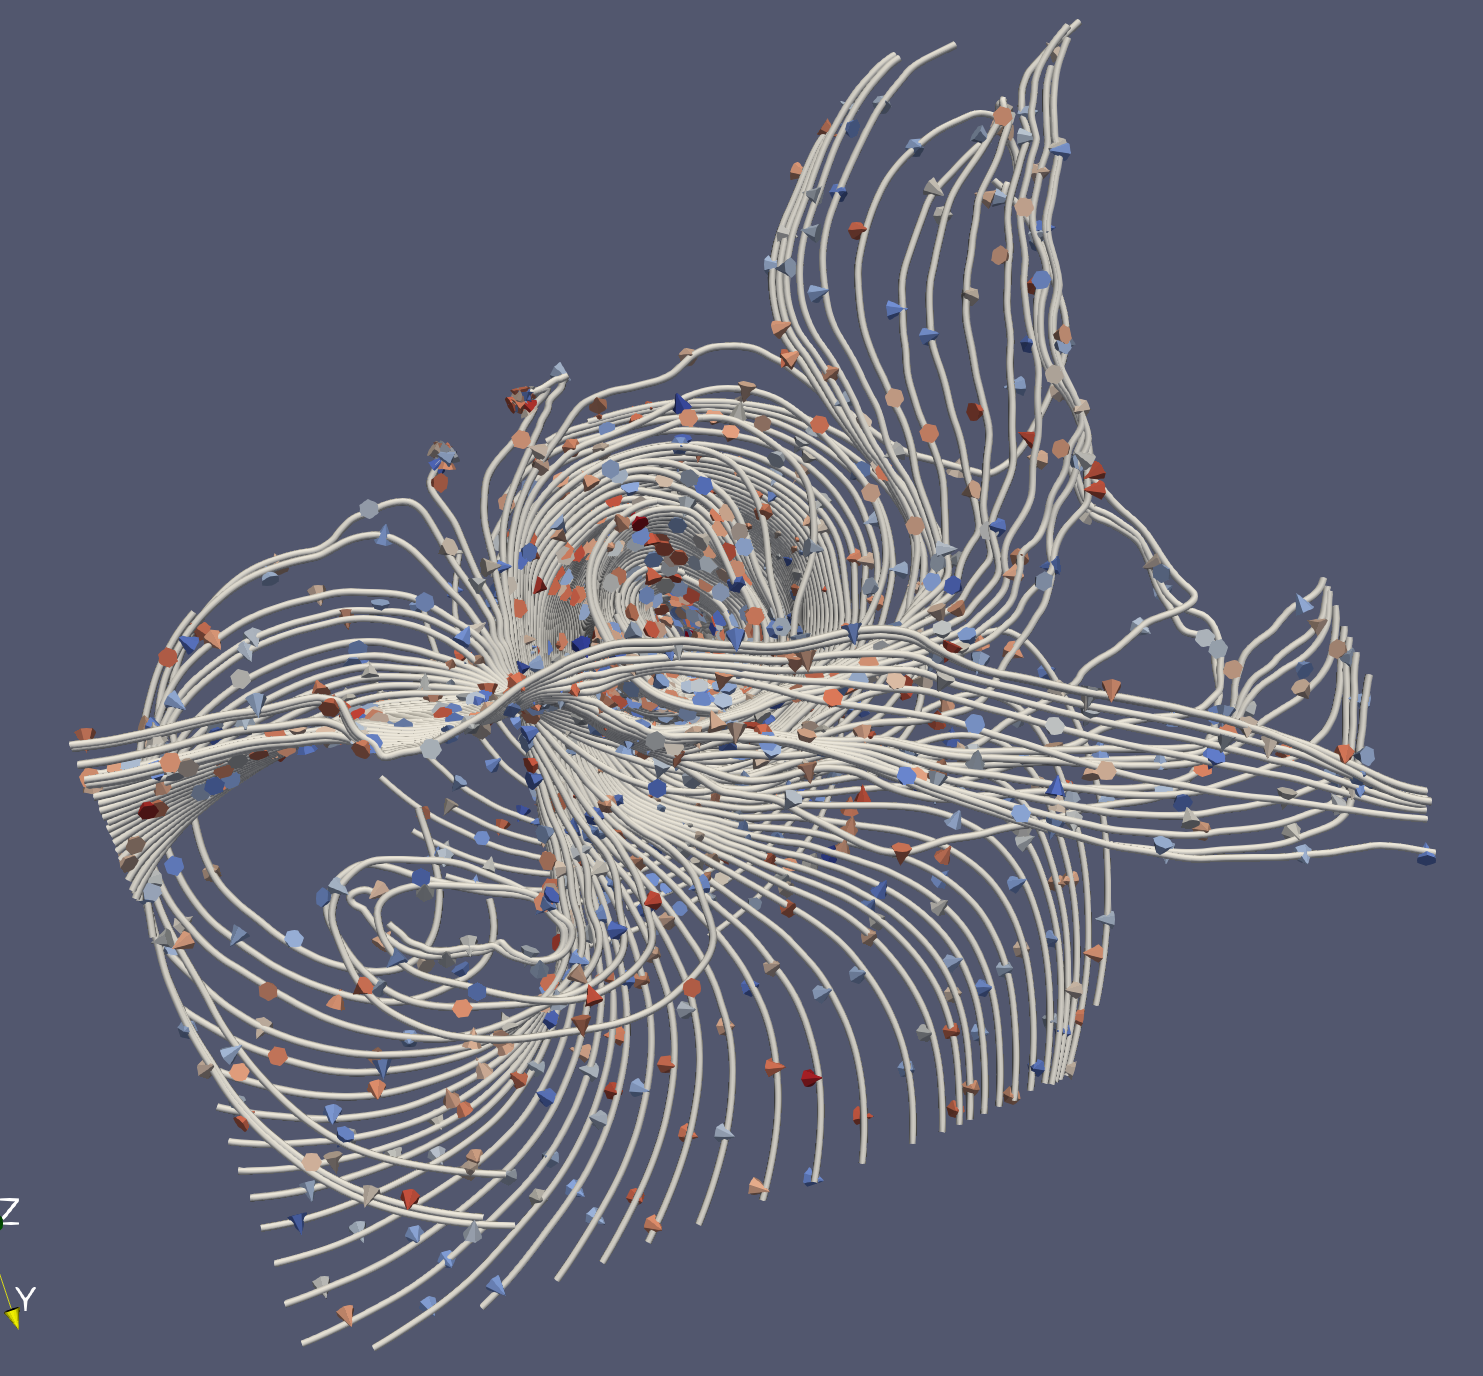
\includegraphics[scale=0.5]{Figures/P2_3_2.PNG}
    \caption{Different views of cone glyphs on top of the Streamtubes}
    \label{p2_3}
\end{figure}
\clearpage
\begin{figure}[!h]
    \centering
    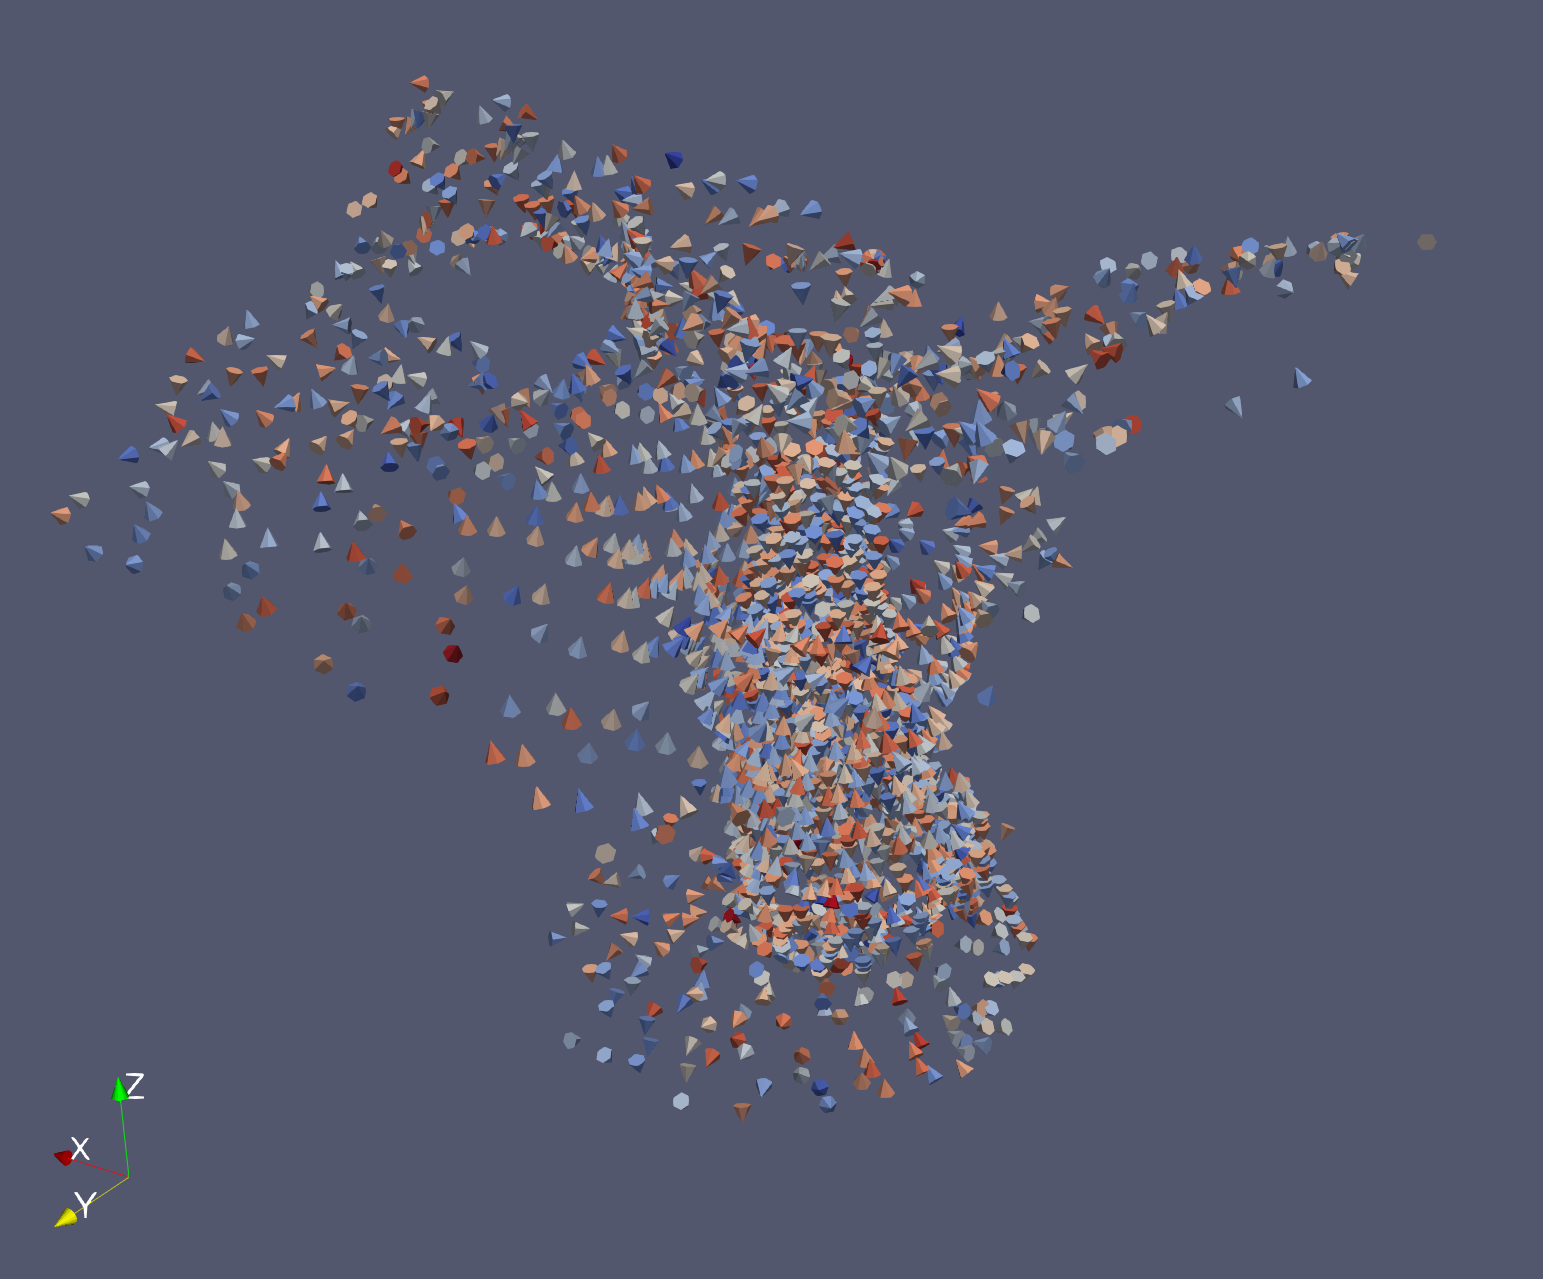
\includegraphics[scale = 0.8]{Figures/P2_3_3.PNG}
    \caption{Cone Glyphs view}
    \label{p2_4}
\end{figure}

\clearpage
\subsection{To see a big picture of the direction of the wind flow within the hurricane, create a visualization using arrow glyphs at randomly sampled places throughout the volume. }
Here, we added a glyph filter to the stream tubes we had. Following the similar settings as previous part here as well. We are using every point out of 800 sampled points i.e. the sampling rate is 800. I also changed the Scale Mode to vector and the scale factor to $\sim$51000. Finally, change the type of glyph to arrow and hit apply. Through this view, we can see the wind flow and directions along the streamlines. For better visualization, I enabled the stream tubes and the glyphs together to get an understanding of the data. From the results attached below we can clearly see the direction of the wind flow and magnitude along the stream tubes. Arrow glyphs allows us to view the direction of wind flow at different locations inside the hurricane. 

\begin{figure}[!h]
    \centering
    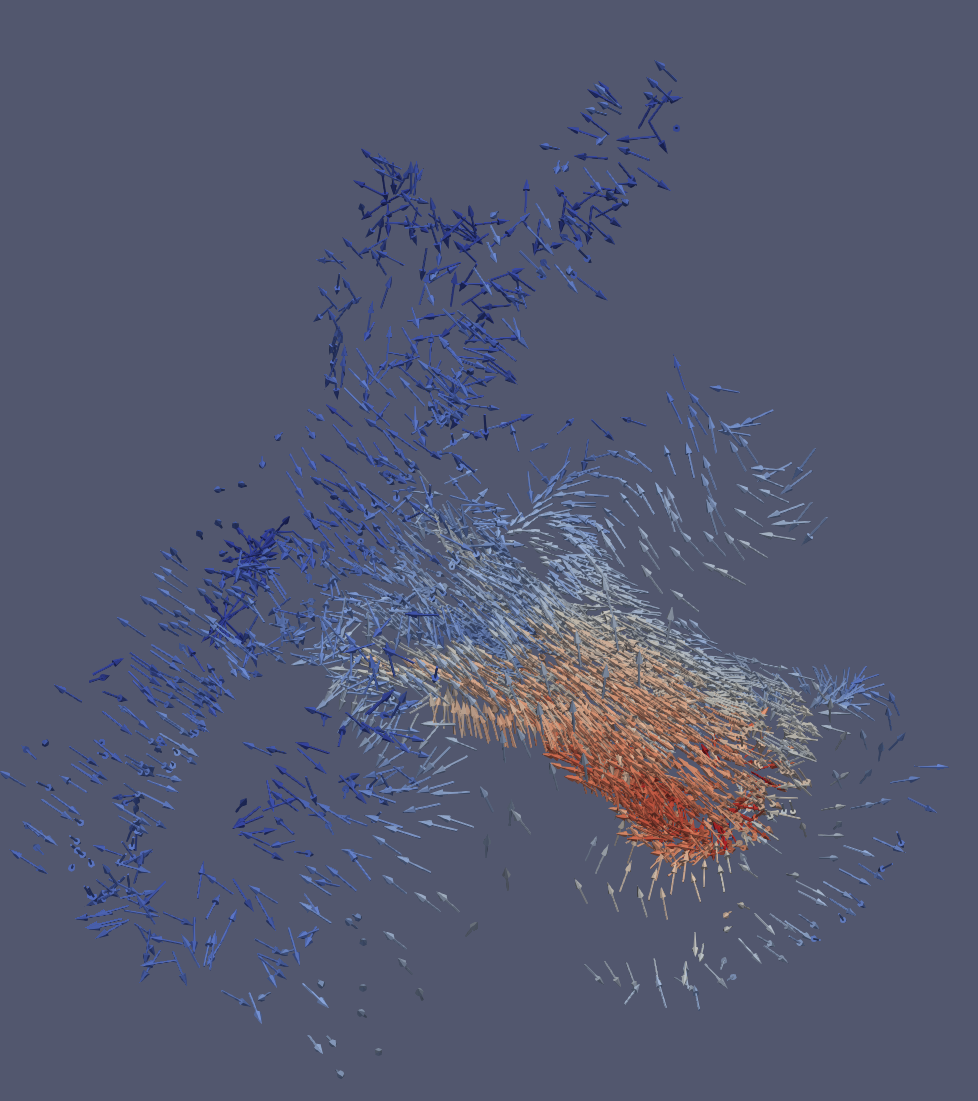
\includegraphics[scale=0.6]{Figures/P2_4_1.PNG}
    
    \vspace{0.5 cm}
    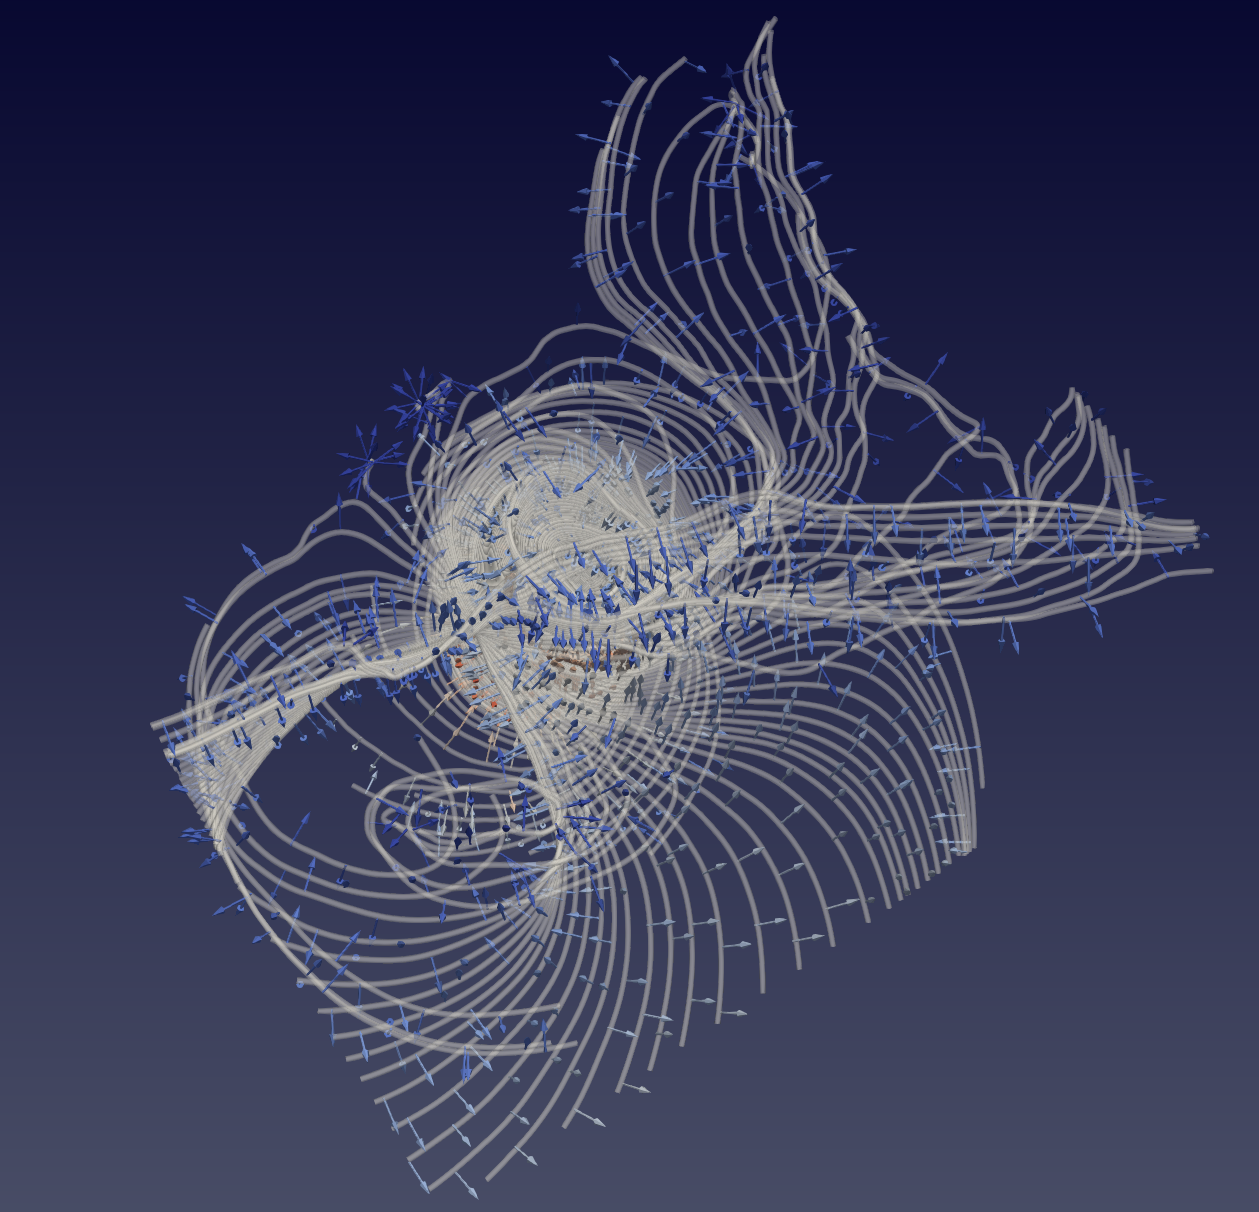
\includegraphics[scale=0.5]{Figures/P2_4_2.PNG}
    \caption{Top: Arrow Glyphs (created on top of the Stream Tube), Bottom: Arrow Glyphs and Stream Tubes together}
    \label{p2_5}
\end{figure}
\clearpage

\begin{figure}[!h]
    \centering
    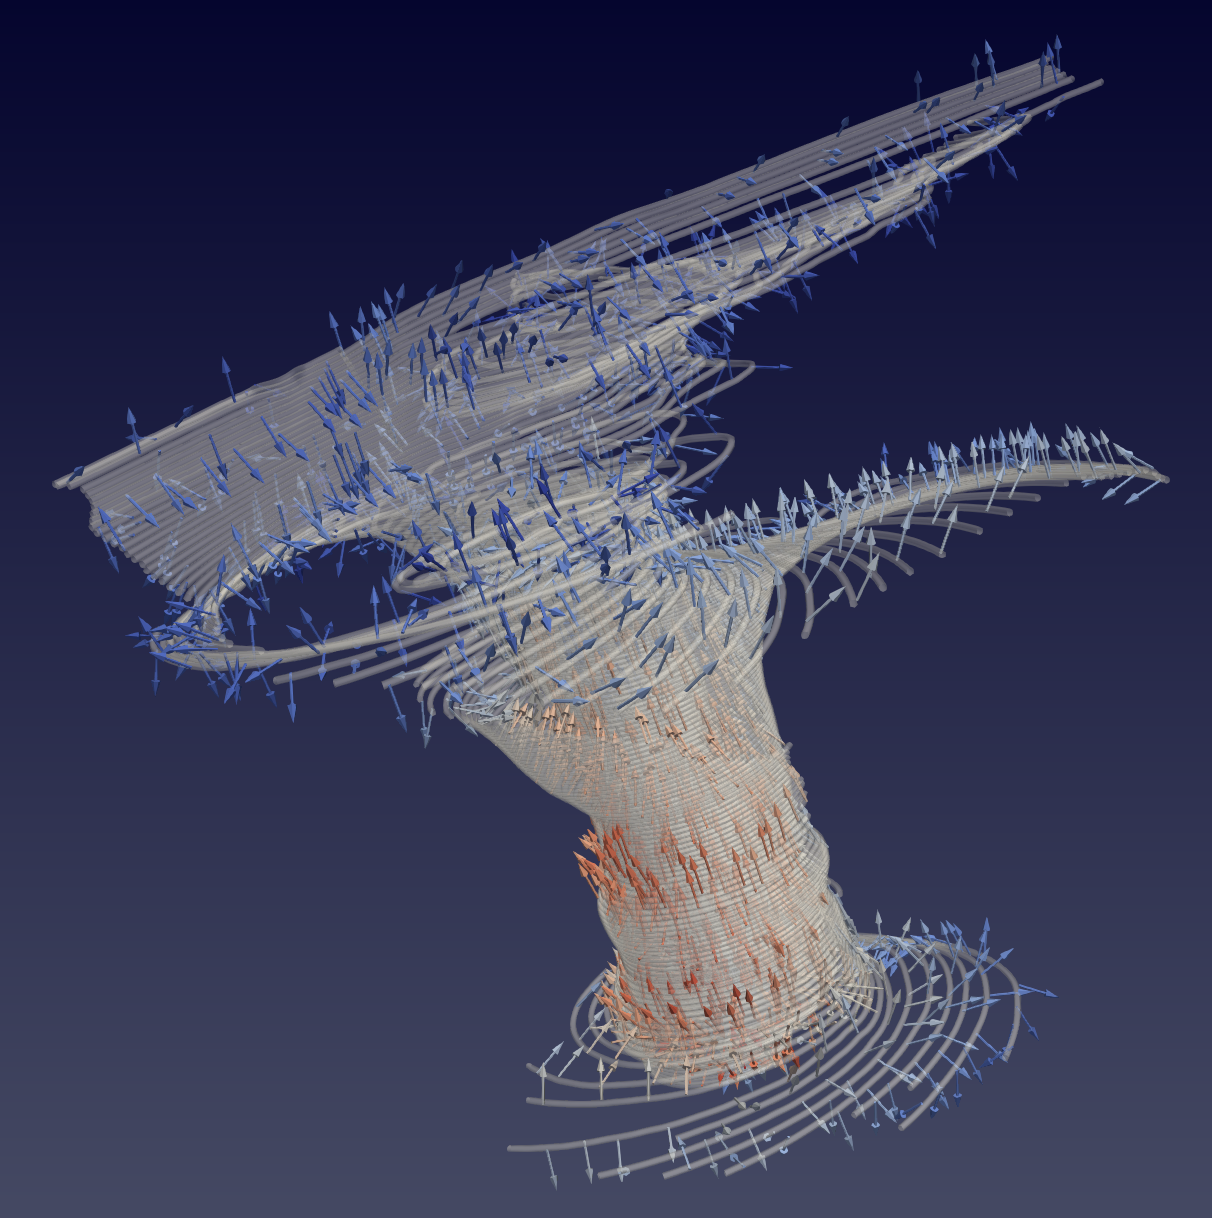
\includegraphics[scale=0.6]{Figures/P2_4_3.PNG}
    \caption{A different view of Arrow Glyphs and Stream Tubes}
    \label{p2_6}
\end{figure}
\clearpage

\section{Multi-Field Visualization}
\subsection{Create a single visualization that includes an isosurface of QCLOUD, plus a volume rendering of QCLOUD, plus streamlines of the wind flow, plus arrow glyphs of the wind flow.}
\paragraph{Ans.} Here, we have to combine the QCLOUD iso-surface, QCLOUD Volume rendering, streamlines, and glyphs together in one view. Here, to make the visualization reasonable, I changed quite a few things. Firstly, I reduced the opacity of QCLOUD isosurface to 0.25. Secondly, I changed the transfer function of Iso-volume rendering to make it more visible with QCLOUD isosorface. Third, I changed the color of Streamlines to Green so as to make it more appealing with others. Finally, I changed the arrow glyph stride to 600 so that there are more arrows. In this view, we get a better understanding and more details about the hurricane dataset. It also help us verify that our simulations are correct or not. For ex. it can be clearly seen that the streamlines of wind follows the qcloud iso-surface and iso-volume. Also, the directions arrow are pointing to gives us a sense of direction which fits well with our intuition as well. I have attached different views for the multi-field visualizations to provide a better understanding to the question. Please find the results starting from the next page. 

\begin{figure}[!h]
    \centering
    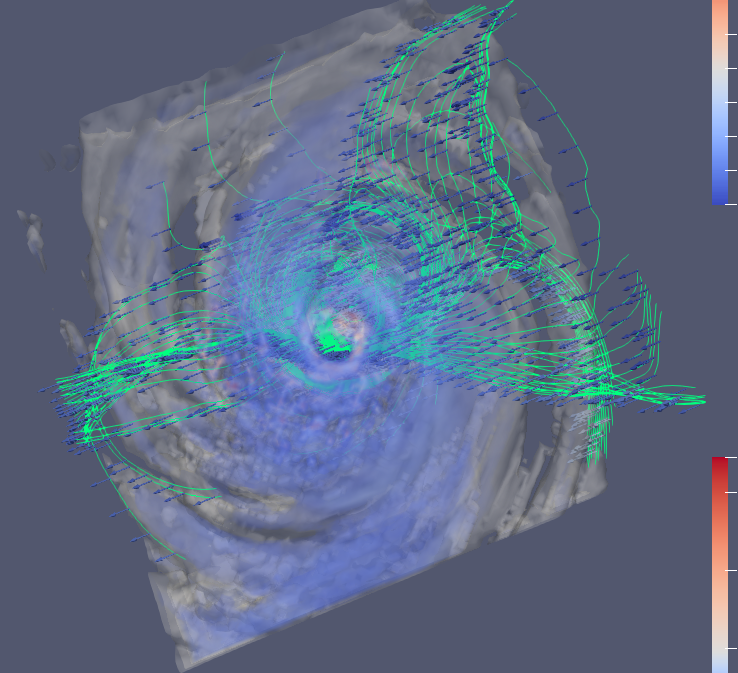
\includegraphics[scale=0.6]{Figures/P3_1.PNG}
    
    \vspace{0.5 cm}
    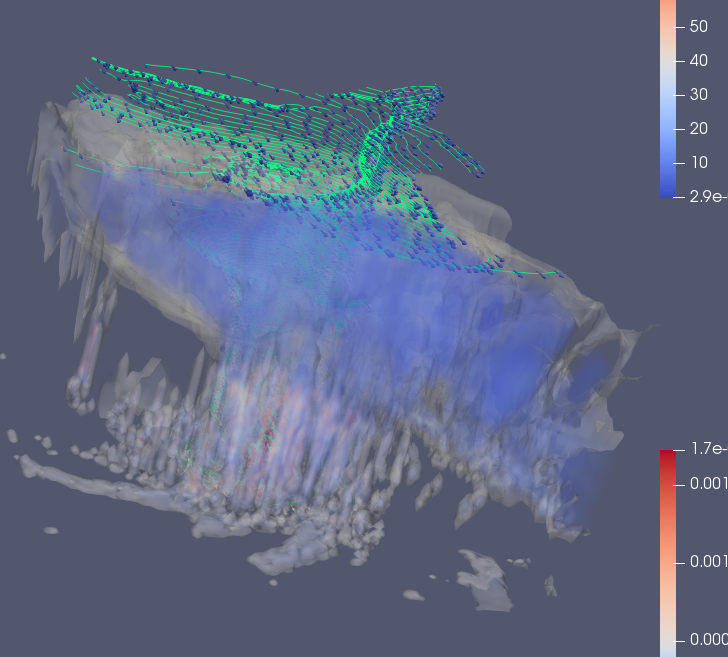
\includegraphics[scale=0.6]{Figures/P3_2.PNG}
    \caption{Different views of Multi-Field Visualization}
    \label{p3_1}
\end{figure}
\clearpage
\begin{figure}[!h]
    \centering
    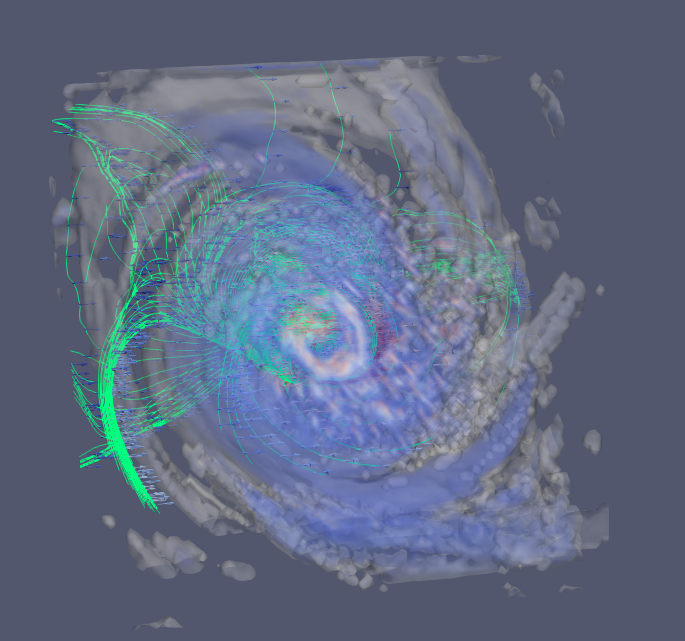
\includegraphics[scale=0.6]{Figures/P3_3.PNG}
    
    \vspace{0.5 cm}
    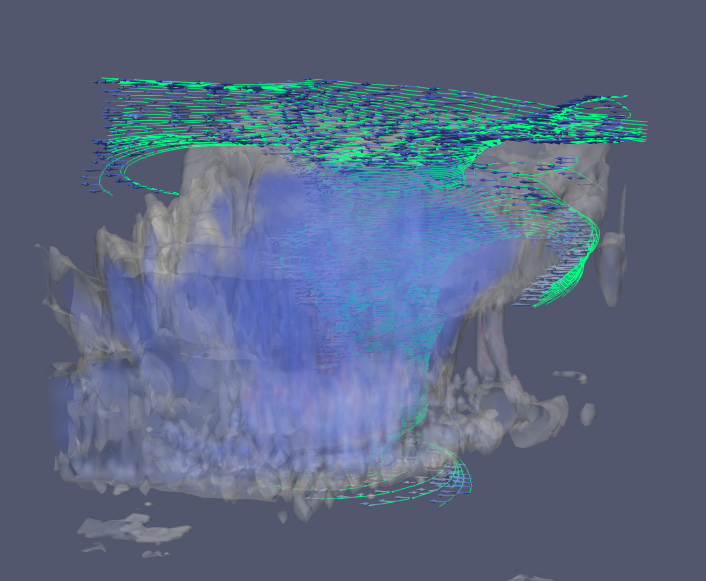
\includegraphics[scale=0.6]{Figures/P3_4.PNG}
    \caption{Different views of Multi-Field Visualization}
    \label{p3_1}
\end{figure}

\clearpage
\section{Discussion and Conclusions}
Frankly, I didn't know how to seperate discussions from conclusions so I decided to create only one section. Here's my experience with this assignment. \\
This assignment gave me a better understanding of how the real world data looks like and how it is visualized. I also learned to interpret important results based on the visualizations. The parameter tweaking in this assignment was very crucial. For example, in the streamline and stream tubes, finding the right value of seed, radius, radius factor etc. was important. Similarly, in part 3, creating a view with multiple fields was a bit difficult. Essentially, finding a right amount of each rendering to use is equally difficult to creating them. At each step, I was wondering that although it looks good but is it good enough for a visualization researcher to draw some significant results or not. Through this assignment, I developed a deeper understanding of the Paraview software and the power of it. I now know why it is one of the best tools for scientific visualization.  
\section{References}
\begin{enumerate}
    \item ParaView Tutorials and Handbook
    \item WRF Website for information on Katrina Dataset
\end{enumerate}
\end{document}